\chapter{Introduction}
\label{cpt:introduction}

In this chapter, we will first introduce chip multiprocessors and their memory systems.
We will also introduce the role of a cache management algorithm, and introduce a set of common memory access patterns.
Then, we will analyze our problem description and introduce a set of requirements the thesis has to fulfill.
Finally, an overview of our contributions is given before we provide an outline of the thesis.

\section{Chip Multiprocessors}

Moore's Law~\cite{Moore1998}, an observation made by G. E. Moore one of the co-founders of Intel, has been the driving force behind processor development in the last decades.
The law is simply an observation; that scaling of transistors used to make integrated circuits will allow for approximately twice the number of transistors per die every 18 months.
Up until the mid-2000s, manufacturers used these smaller transistors to increase single-core performance.
Smaller transistors allowed for increased frequency, and more transistors per die allowed for increasingly complex processor cores.
Features such as speculative and out-of-order execution were added to take advantage of instruction-level parallelism (ILP) present in computer programs.
By the mid-2000s, processor cores had become so complex and were running at such high frequencies that manufacturers had reached the limitation known as the power wall.
The power wall entails that manufacturers were unable to continue increasing the frequency and the transistor count of each core, without also attaching high-performance cooling systems to counter the increased power usage and hence increased heat generation.
Systems like water or even nitrogen cooling were needed to continue the single core performance increase~\cite{Sutter2005}; these systems are not practical for personal computers.

Figure~\ref{fig:introduction:memgap} shows the single core performance development from 1980 to 2010.
The effect of the power wall is clearly visible from 2005 and out where we observe no improvement in single core performance.
We also observe that in the five years leading to the power wall, the yearly performance improvement decreased.
This decrease is observed because improving single core performance became harder, as more advanced techniques for ILP exploiting where needed, ultimately resulting in the power wall.

\begin{figure}[ht]
\centering
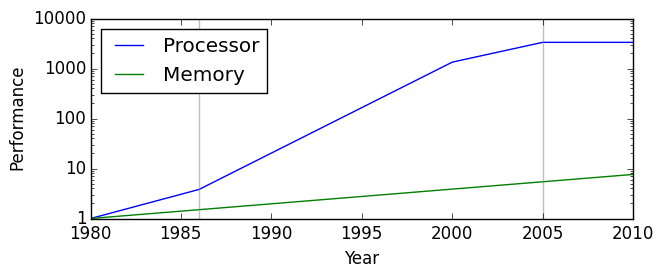
\includegraphics[width=.8\textwidth]{figures/introduction/memory-gap}
\caption[Processor-Memory Gap]{Comparison of (single core) processor and memory performance from 1980 to 2010 based on data collected by J. Hennessy and D. Patterson~\cite{hennessy2012}.}
\label{fig:introduction:memgap}
\end{figure}

By 2005, most manufacturers had abandoned their plans for increased single core performance and were all working towards chip multiprocessors (CMPs)~\cite{Sutter2005}.
CMPs are built using several simpler processing cores without many of the aggressive ILP utilization features that were added to single core processors in the late 2000s to increase performance.
This development is based on Pollack's rule~\cite{Borkar2007}, which states that performance increases proportionally to the square root of the area, and that power usage increases proportionally to the area.
Consider having two cores, one large highly complex core, and a simpler core at half the size.
The performance of the larger core will by Pollack's rule be worse than the combined performance\footnotemark of the two smaller while having roughly the same power consumption.
\footnotetext{Single thread performance is only increased by creating more complex cores; multithreading techniques are required in software to take advantage of CMPs performance increase.}
Moving to simpler and smaller cores allowed manufacturers to continue overall performance improvements while keeping below the power wall.
With an increasing number of transistors due to scaling, even more processing cores can be added to CMPs.
Today CMPs are the de-facto standard, being used in everything from embedded computers~\cite{ARM2010} and mobile phones~\cite{Ho2014} to commercial and high-performance computing~\cite{Thomadakis2011, Jain2013}.


\section{CMP Memory System}

Memory is a vital component of any computing system, without memory we are unable to store our programs and computations.
Traditionally the technology used to create memory have differed from the technology used in processors~\cite{Wilkes2001}.
As processor performance increased, memory performance did not increase proportionally.
This development has resulted in what is known as the processor-memory gap~\cite{Wilkes2001}.
Figure~\ref{fig:introduction:memgap} shows how the gap in processor and memory performance has developed from 1980 to 2010.
The figure shows that memory performance has had a constant development over the period of about 7\% increase yearly.
The processor-memory gap made itself visible in 1986 when processor performance started increasing by about 52\% each year.
If not handled, the increasing processor-memory gap would become the limiting factor in processor performance, as processors are dependent on the memory system providing both code and data.
In response to the growing gap small and fast memory structures known as caches were introduced.
Caches are produced using different techniques than main memory, proving faster access. 
This comes at the cost of higher production cost and power usage.
Today, most single-core processors and CMPs have one or more caches integrated on the processor die.
The caches filter all memory request made by the processing core.
If one of the caches has a copy of the requested data, it will stop the memory request from going to main memory and respond with the correct data.
This is known as a cache hit.
If a cache does not have the value of the requested address, it is known as a cache miss.
Because caches are faster and are located closer to the processor than main memory they can to an extent hide the processor-memory gap, assuming a high hit rate in the caches.

\begin{figure}
    \centering
    \begin{subfigure}[b]{0.45\textwidth}
        \centering
        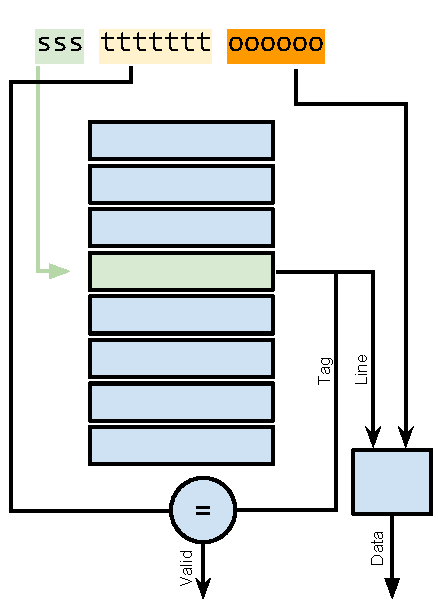
\includegraphics[width=.7\textwidth]{figures/introduction/dircache_read}
        \caption{Direct mapped cache. Each set contains only one block. The three most significant bits used for set addressing, 7-bit tags.}
        \label{fig:introduction:cache:dir}
    \end{subfigure}\hfill%
    \begin{subfigure}[b]{0.45\textwidth}
        \centering
        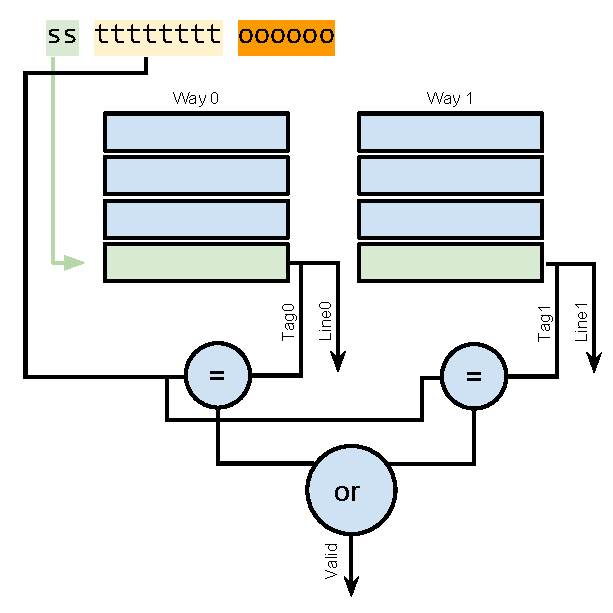
\includegraphics[width=.8\textwidth]{figures/introduction/2waycache_read}
        \caption{2-way associative cache. Each set contains two blocks. Two bits used for set addressing, 8-bit tags. Additional hardware (not shown) required to select output between line0 and line1.}
        \label{fig:introduction:cache:2way}
    \end{subfigure}
    \caption[Direct mapped and 2-way cache architecture.]{Simplified architecture of a direct and 2-way cache under a read operation. With 64B lines and byte addressing.}
    \label{fig:introduction:cache}
\end{figure}

Traditionally there are three main ways of organizing cache memory; direct mapped, set associative and fully associative.
Caches used in commercial CMPs today are set associative memory structures~\cite{Thomadakis2011, Jain2013, ARM2010, Ho2014}.
A cache is organized as a 2d array, where each row is called a set, and each set consist of one or more blocks, sometimes known as cache lines.
A block is the minimum unit of data a cache stores, this is typically 64B.
The cache divides all memory addresses into three portions, the set address, block tag and block offset.
The set address is used to determine which set is responsible for caching a value.
Within a set, all blocks are valid storage locations.
Each block that contains valid data also stores the block tag of the data it contains.
During a cache lookup, all valid blocks will be scanned looking for one containing the block tag from the address.
In a direct mapped cache, each set contains only one block, making the block scan trivial.
Fully associative caches have all blocks in a single set, and the block scan require that every block be checked.
This is expensive both measured in hardware required, and the critical path of the cache.
Set associative caches, also known as n-way caches, are a middle ground organization that stores n blocks per set.
Figure~\ref{fig:introduction:cache} shows both a direct mapped and a 2-way cache under a read operation.
The figure does not show a fully associative cache organization but given the 2-way cache organization a fully associative cache is created by duplicating the block scan hardware until each column has only one row.
In this thesis, we will show that increasing the number of ways can improve performance of a cache via increased hit rate.
However, the access time and complexity of a cache also increases as the number of ways increases.
As a result, first level caches are often limited to 2- or 4-ways~\cite{Sanchez2010}, because the access latency must be short to prevent the CPU stalling while it waits for data. 
Even third level caches rarely exceed 16- or 32-ways.
Alternative cache organizations have been proposed, such as zcache~\cite{Sanchez2010}, that allows for higher associativity while providing access times comparable to traditional caches.
However, these techniques are not currently used in commercial CMPs and hence are not considered further in this thesis.

When data not present in the cache is requested by a processing core, a request is sent to the next cache level, or possibly the main memory.
Once the cache receives a response, it normally stores the data to provide faster access times in case of a re-reference.
Caches also normally store data that is written to memory by a processing core, speeding up the write operation.
For a set-associative or fully associative cache, there are multiple valid storage locations for a data block.
An algorithm known as the cache management algorithm decides which of the valid blocks are used to store the value.
If the block that was chosen by the algorithm already contains valid data the cache removes or evicts the existing data.

\begin{figure}[th]
\centering
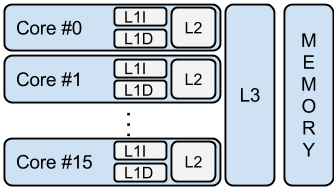
\includegraphics[scale=.65]{figures/processor_model/processor_model}
\caption{Generic Chip Multiprocessor Architecture.}
\label{fig:cmp_model}
\end{figure}

In the memory hierarchy, smaller means faster. 
For instance, main memory is much faster than disks, but disks can store much more data.
The same is valid for caches, a smaller cache has a shorter critical path and hence a lower access time compared to a larger cache.
Figure~\ref{fig:cmp_model} shows an example 16-core CMP architecture with three cache levels and main memory.
For each cache level, both the size and access time increases.
First level caches are the smallest while the third level caches are largest.
To save area on CMPs, and also to provide an easy mechanism for data sharing between cores, it is common to have at least one level of shared cache.
In Figure~\ref{fig:cmp_model} each core has a private L1 and L2 cache, and a shared last-level cache (LLC), the L3 cache.
While sharing cache can improve performance, and improve overall utilization, it also makes the memory system exposed to destructive interference that potentially can hurt the performance of all processing cores. 
The cache management algorithm, running on the shared cache, may either ignore the effects of interference or it may attempt to reduce it by some form of prioritization.

\section{Common Memory Access Patterns}

In this section, we will define four memory access patterns~\cite{Jaleel2010}; recency-friendly, trashing, streaming and combined access patterns.
These patterns will later be used to describe the strengths and weaknesses of the presented algorithms, and to explain algorithm performance in our experiments.

\subsection{Recency-friendly}
Several cache management algorithms make an assumption known as the recency-assumption.
This is the assumption that recently accesses memory addresses have a higher probability of re-use that less recently accesses addresses.
A recency-friendly access pattern is one that causes no misses under an algorithm that always keeps the most recently used blocks in the cache.
Figure~\ref{fig:algorithms:rf_pattern} illustrates an example memory access pattern that is said to be recency-friendly.
Because the pattern repeats and $k$ is less than the number of ways we know that the least recently used block will always be referenced before being evicted, if we assume a recency-assumption based algorithm.
Hence, the algorithm will be able to provide hits for every access after the initial repetition and the pattern is recency-friendly.

\begin{figure}[ht]
\centering
$p_{rf} = (a_0 a_1 ... a_{k-1})^N$
\caption[Recency-friendly access pattern.]{Recency-friendly access pattern (k $<=$ number of ways, N $>$ 1).}
\label{fig:algorithms:rf_pattern}
\end{figure}

\subsection{Trashing}
A trashing memory pattern is one that repeats in a similar manner to a recency-friendly pattern, but with more blocks per cycle than the number of cache ways. 
Figure~\ref{fig:algorithms:tr_pattern} shows an example of one such pattern, the only thing separating this from the previous pattern in the value of $k$.
Under a recency-assumption based algorithm, an access pattern similar to this will never hit because all blocks are evicted before they are re-referenced.
A better management algorithm for these patterns might keep some of the working set in the cache, providing hits for parts of the access pattern.
\begin{figure}[ht]
\centering
$p_{rf} = (a_0 a_1 ... a_{k-1})^N$
\caption[Trashing memory access pattern.]{Trashing memory access pattern (k $>$ number of ways, N $>$ 1).}
\label{fig:algorithms:tr_pattern}
\end{figure}

\subsection{Streaming}
A streaming memory access pattern is one that has no re-references, or where the period is so large that no pattern is detectable.
Figure~\ref{fig:algorithms:st_pattern} illustrates one such pattern, where k is infinite.
No caching algorithm can provide hits for such an access pattern, simply because there are no re-references.

\begin{figure}[ht]
\centering
$p_{rf} = (a_0 a_1 ... a_{k-1})$
\caption[Streaming memory access pattern]{Streaming memory access pattern (k = $\infty$).}
\label{fig:algorithms:st_pattern}
\end{figure}

\subsection{Combined}
In reality, memory access patterns can be more complex than the simple examples shown above.
A single program might, for instance, behave both in a recency-friendly and streaming fashion. 
An example would be a program performing a reduction over a large dataset.
Most accesses would be streaming as the program iterates over the dataset, but some accesses will exhibit recency-friendly behavior like when the program stores temporary results to memory during the iteration.

For shared caches, the observed pattern is the union of accesses from all cores.
A particular non-optimal situation for a cache assuming recency-friendly behavior is when multiple cores execute recency-friendly applications, and one single core execute a streaming application.
In this case, the streaming application will constantly clear the cache, degrading performance of the recency-friendly applications.
An algorithm that could detect the streaming application and handle it as a special case could potentially increase the performance of the recency-friendly applications without affecting the performance of the streaming application.
Some of the algorithms we cover in the following sections will attempt to detect streaming applications.

\section{Requirements}
By analyzing the problem description, we have been able to extract a set of requirements that this thesis has to fulfill:

\begin{description}
    \item[R1] Introduce CMPs, their memory system, and the role of a cache management algorithm.
    \item[R2] Present recent and important work in the cache management field. Compare similarities and differences of the various proposed algorithms.
    \item[R3] Create a framework for evaluation of various cache management algorithms.
    \item[R4] Implement at least one of the presented algorithms and compare against a conventional LRU-managed cache.
\end{description}
Based on the problem description and discussions with the thesis advisors, we list an additional set of optional requirements that the thesis may fulfill:

\begin{description}
    \item[O1] Implement additional algorithms and evaluate them.
    \item[O2] Compare performance of the implemented algorithms against each other.
    \item[O3] Investigate algorithm sensitivity to changes in L2 cache size, L3 cache size, and/or memory bus bandwidth.
\end{description}

\section{Contributions}

In our work with this thesis we have made the following contributions:

\begin{itemize}
  \item We have created a curated list with detailed descriptions of several recently published algorithms in the cache management field. The list has been limited to only consider algorithms that target conventional caches and optimize for cache miss minimization.
  \item A framework for evaluation of cache management algorithms has been built on top of the Sniper~\cite{Carlson2011a} simulation system.
  \item Several of the algorithms presented in our list of existing works have been implemented and tested within our simulation framework.
  \item We performed several sensitivity experiments further exploring the properties of our simulation framework and the implemented algorithms.
  \item The implemented simulation framework and all our results will at the end of this thesis be made available to NTNU and the CARD~\cite{CARD2015} research group for future research.
\end{itemize}

\section{Outline}

The outline of the rest of this thesis is as follows:

\begin{itemize}
  \item Chapter~\ref{cpt:introduction} introduces the thesis by putting it in a historical context, presenting important background knowledge and summarizing the contributions made, fulfilling requirement \textbf{R1}.

  \item Chapter~\ref{cpt:algorithms} presents a selection of cache management algorithms and provides a theoretical comparison of them, fulfilling requirement \textbf{R2}.

  \item Chapter~\ref{cpt:framework} presents our simulator and the framework built on this simulator to enable evaluation of cache management algorithms. It also presents the subset of algorithms we have implemented. This fulfills requirement \textbf{R3} and \textbf{O1}.

  \item Chapter~\ref{cpt:methodology} contains a description of our simulated processor model and explains all metrics we later use to evaluate our experiments.

  \item Chapter~\ref{cpt:results} presents an experiment where we compare all implemented algorithms against an LRU managed cache. Also, we compare all implemented algorithms against each other. This fulfills requirement \textbf{R4} and \textbf{O2}.

  \item Chapter~\ref{cpt:sresults} presents five different experiments all exploring either simulation framework or algorithm sensitivity to various architectural changes, fulfilling requirement \textbf{O3}.

  \item Chapters~\ref{cpt:discussion} and~\ref{cpt:conclusion} contain a discussion of our results and a conclusion based on these. Also, an overview of future work is given.

\end{itemize}